\part{Materiais e Métodos}
	\chapter{Reagentes}
	
	Os reagentes utilizados, suas respectivas purezas e os fabricantes se encontram na tabela \ref{tab:reagentes}.
	
	\begin{table}[H]
		\IBGEtab%
		{\caption{Reagentes, pureza e fabricantes}
		\label{tab:reagentes}}%
	    {
		\centering
		\begin{tabular}{c c p{3.2cm}}
			\toprule
			Reagente  & Pureza                                      & Fabricante    \\ \midrule
			  CTAB    & $\geqslant 98\%$                            & Sigma Aldrich \\
			  TTAB    & $\geqslant 99\%$                            & Sigma Aldrich \\
			  DTAB	  & $\geqslant 98\%$							& Sigma Aldrich \\
			  NaSal   & $99{,}5\%$                                    & Sigma Aldrich \\
			Glicerina & $85\%$/$15\%\textnormal{H}_2\textnormal{O}$ & Merck         \\
			Sacarose  & $\geqslant 99{,}5\%$                          & Sigma Aldrich \\
	%		Sucralose & 											& 				\\  % todo: ver se coloco algo da sucralose aqui
			  Ureia   & $\geqslant 99{,}5\%$                          & Sigma Aldrich \\
			  DMSO    & $\geqslant 99{,}5\%$                          & Sigma Aldrich \\
			  1,3BD   & $99{,}5\%$                                    & Sigma Aldrich \\ 
			  Água    & $\sigma = 18{,}2M\Omega$.cm					& Millipore Direct-Q\textregistered{} \newline 3 UV com bomba  \\ \bottomrule
		\end{tabular}}%
		{}
	\end{table}
	
	\chapter{Reologia}
		\section{Preparo das amostras}
		\label{sec:reologia_preparo_amostra}
		O preparo de amostras de reologia deve ser feita de modo a garantir a completa homogeneização, e perda de memória reológica da amostra. A densidade do solvente é utilizada para os cálculos de concentração, para se determinar as concentrações, em \mM, do surfactante e de NaSal. Não foi considerada a alteração de densidade pela adição de surfactante e NaSal, somente dos aditivos.
		
		Após a pesagem dos componentes em balanças de precisão, frequentemente partindo de soluções estoque altamente concentradas, as amostras são aquecidas até 50°C em banho maria e homogeneizadas por meio de agitação manual e com vórtex. Temperaturas elevadas auxiliam na dissolução dos componentes e diminuem a viscosidade do meio, por também desfavorecerem o crescimento das micelas. Após já homogeneizadas, as amostras são mantidas a 50°C, e depois são resfriadas lentamente até temperatura ambiente removendo-se o aquecimento do banho maria. Neste instante, as amostras estão prontas para análise reológica. As amostras eram preparadas no mínimo com 24h de antecedência.
		
		\section{Análises reológicas}

		% todo: checar se só foi utilizado esse reômetro
		Todas as análises reológicas foram realizadas utilizando a geometria placa-placa de 35 mm de diâmetro (P35 Ti L) no reômetro Haake Mars III da Thermo Scientific. Antes de cada análise, a inércia do porta-rotor (\emph{spindle}) e do rotor eram determinadas de modo a controlar por erros relacionados ao encaixe manual do rotor. Também era determinado o ponto zero de altura, onde há o contato do rotor com a base, de modo a estabelecer um espaçamento de 1,000 mm durante as análises. A temperatura era controlada pela combinação de um banho termostatizado e de aquecimento na base, e monitorada por meio de sensores na base.
		
		As amostras são transferidas para a placa do reômetro simplesmente vertendo-se os tubos falcon até que a área de análise estivesse coberta. Caso as amostras fossem resistentes demais, uma espátula era utilizada para cortar e espalhar o gel sobre a base. Em seguida, o rotor era abaixado e observava-se se não havia falta de amostra em algum ponto. Caso houvesse falta, a amostra era recuperada e reaplicada na base. O cisalhamento causado pela transferência de amostra e pelo abaixamento do rotor não foram levados em consideração nas análises. A amostra era coberta por um protetor de teflon de modo a minimizar a perda de solvente durante a análise.
		
		Os métodos de análise são montados de acordo com as necessidades de cada amostra. Em comum, somente há a etapa de termostatização por 5 minutos na temperatura de análise. As etapas possíveis são:
		
		\begin{itemize}
			\item Análise de varredura de tensão. A faixa de valores de tensão estudados foram geralmente de 0,01 Pa até 5 Pa, espaçados logaritmicamente, analisados a 1 Hz. Com essa análise é possível determinar a região linear, onde os valores de G' e G'' estão constantes, independente da tensão aplicada. Caso uma tensão alta demais seja aplicada, começa a ocorrer a desestruturação do material, e os valores de G' e G'' diminuem.
			
			\item Análise de varredura de frequência, numa tensão dentro da região linear, geralmente 1 Pa. A faixa de frequência estudada varia de acordo com as necessidades da amostra e com o tempo disponível, pois quanto menor a frequência estudada, maior é o tempo de análise. A faixa de frequência habitual é de 0,01 Hz a 10 Hz (ou 0,0628 rad.s\menosUm{} a 62,83 rad.s\menosUm), e 6 medidas por década, espaçadas logaritmicamente. Este tipo de experimento demora cerca de 20 minutos. O modo utilizado em todas as análises foi CS (Control Shear).
			
			\item Análise de curva de fluxo. As taxas de cisalhamento ($\dot{\gamma}$) utilizadas geralmente variavam de 0,001 s\menosUm{} a 10 s\menosUm. Caso o platô Newtoniano não fosse observado, diminuia-se a taxa aplicada. Obtinha-se entre 10 e 20 pontos espaçados logaritmicamente. As medidas eram obtidas no modo CR (Control Rate).
		\end{itemize}
		
		Ao montar-se um plano experimental, pode-se configurar o equipamento para exportar os dados obtidos de acordo com uma configuração tabular específica, para um arquivo de texto. Isso facilita posteriormente o tratamento de dados. Além disso, o nome do arquivo pode ser gerado automaticamente pela composição da amostra, a hora e a data de análise.
		
		\section{Tratamento de dados de reologia oscilatória}
		
		Para micelas gigantes, a obtenção de informações microscópicas da amostra geralmente é realizada através de um ajuste das curvas de G' e G'' ao modelo de Maxwell. Com esse ajuste, é possível obter informações como o tempo de relaxação estrutural das micelas e os módulos elásticos das soluções. Para realizar o tratamento, os dados foram importados ou para o software Origin\textcopyright{} 9 ou Python, e o modelo de Maxwell foi ajustado para G' e G'' utilizando-se um conjunto de parâmetros para ambas as curvas, obtidos pelo método dos mínimos quadrados.
		
		A região utilizada para os ajustes depende da qualidade subjetiva dos pontos. Por exemplo, em altas frequências de oscilação, a confiabilidade dos valores de G' e G'' é menor devido à inércia do rotor. Por essa razão, há muito ruído em altas frequências, e a região de ruído varia de amostra para amostra. Dessa maneira, cada dado é analisado separadamente, removendo-se os pontos ruidosos.
		% todo: colocar referência das seções relevantes.
		% todo: quando eu analisar novamente os dados de reologia oscilatória das amostras com aditivos, onde eu farei também análises de Cole Cole e descobrirei outros tempos de relaxação, colocar aqui como que esses métodos foram feitos
		
		\section{Tratamento de dados de curvas de fluxo}
		
		Micelas gigantes são fluídos conhecidamente pseudoplásticos, ou seja, sua viscosidade aparente ($\eta$) diminui com o aumento da taxa de cisalhamento ($\dot{\gamma}$). Em baixos valores de $\dot{\gamma}$, a viscosidade aparente é constante, e esse valor é chamado de viscosidade no repouso, $\eta_0$. Esse valor é de maior interesse para este trabalho. Para obter esse valor, é possível realizar ajustes lineares da região onde a viscosidade é constante, forçando-se a inclinação da reta a zero. Em suma, isso obtém o valor médio da viscosidade no repouso. Há também modelos matemáticos que podem ser usados, como Carreau e Cross, e a viscosidade no repouso, dentre outros parâmetros, podem ser obtidos pelo método dos mínimos quadrados.
		
		Dados de curva de fluxo também são passíveis de desvios, que dificultam os ajustes. Nas amostras observadas aqui, geralmente há problemas em baixas taxas de cisalhamento. Para contornar esse problema, é necessário selecionar uma faixa de valores para o ajuste, o que pode ser feito manualmente e programaticamente. O apêndice \ref{sec:apn_tratamento_CF} mostra brevemente como o programa para tratamento de curva de fluxo funciona, os problemas frequentes encontrados com curvas de fluxo e como contorná-los.
		
	\chapter{Calorimetria de titulação isotérmica}
		\section{Preparo de amostra e uso do equipamento}
		\label{sec:preparo_amostra_itc}
		% todo: verificar qual é a variação de volume
		
		Na calorimetria de titulação isotérmica (ITC), titula-se uma solução contida numa seringa em outra solução contida numa cela. Esse processo pode liberar ou absorver calor, e a quantidade de calor absorvido ou liberado é dependente de todos os processos que ocorrem durante a injeção, por exemplo, diluição e micelização. Essa sensibilidade exige que muito cuidado seja tomado na preparação de amostra, de modo a obter soluções bastante limpas e homogêneas, sem interferentes, e com concentração bem conhecida. Além disso, o solvente de ambas as soluções (da seringa e cela) devem ser estritamente os mesmos, para impedir que exista um sinal de mistura do solvente.
		
		Quando o solvente das amostras é diferente de água, prepara-se inicialmente a quantidade necessária de solvente para todas as amostras, e esse solvente é utilizado tanto para as soluções da cela quanto da seringa. Após isso, os componentes sólidos são adicionados às soluções, que são homogeneizadas e depois ficam em repouso por no mínimo 24 horas. Variações de densidade são somente consideradas na formação do solvente binário, e não são consideradas nas outras etapas pois a concentração das espécies é menor. As soluções foram preparadas em tubos falcon previamente limpos com etanol, água de torneira e água deionizada três vezes.
		
		A escolha das concentrações das espécies na cela e na seringa dependem do sistema que será estudado, e da região do entalpograma que se deseja observar. Neste trabalho, o sistema de referência é uma solução 1,5 \mM{} de NaSal na cela e TTAB 14 \mM{} na seringa, com água deionizada como o solvente em comum. Esse sistema permite a observação do início dos entalpogramas, antes da micelização, a formação de micelas gigantes e o início da região de transformação para micelas esféricas. Caso se deseja observar o perfil completo, é necessário aumentar a concentração de TTAB, porém perde-se resolução e o início do entalpograma. Caso o solvente seja alterado, é necessário realizar medidas prévias para determinar a melhor concentração de surfactante para a região que se deseja observar.
		
		% todo: achar certinho os volumes e colocar aqui.
		Neste trabalho, utilizou-se tanto o VP-ITC da Microcal quanto o PEAQ-ITC da Malvern. A diferença entre esses sistemas é, essencialmente, o volume da seringa e da cela, que é menor no PEAQ-ITC. A limpeza deve ser feita antes de qualquer análise.
		
		Para a limpeza do VP-ITC, lava-se a seringa internamente com aproximadamente 15 mL de etanol, seguido de 25 mL de água deionizada. A cela é limpa preenchendo-se a cela 5 vezes com etanol, e em seguida 500 mL de água deionizada recém preparada é passada continuamente pela cela por meio de um sistema de vácuo. Após isso, remove-se o restante de água na cela, e coloca-se a solução na cela, tomando cuidado para remover bolhas e o excesso de solução. A seringa é seca, passando-se ar por seu interior, e depois é preenchida com sua solução e o conteúdo é purgado e repreenchido duas vezes. Caso seja necessário, é possível colocar Contrad 70 20\% na cela e aumentar a temperatura até 50°C por algumas horas para remover alguma sujeira resistente, como proteínas.
		
		% todo: checar se o Soak é a 50°C.
		A limpeza do PEAQ-ITC é feita automaticamente pelo equipamento, com três modos disponíveis. Para medidas de rotina, utiliza-se somente a função \emph{Rinse}. Nesse modo, passa-se somente água na cela e na seringa, água é inicialmente passada, seguido de metanol, para auxiliar na secagem. Caso o sistema precise de uma limpeza mais profunda, por exemplo, se polímero ou proteína foi utilizado num experimento anterior, utilizou-se o método \emph{Wash}, que usa Contrad 70 20\% para limpar a cela. Em casos extremos, utilizou-se a função \emph{Soak}, onde uma solução de Contrad 70 20\% é colocada na cela por 1h a 50°C. A cela e a seringa são preenchidas da mesma maneira que no VP-ITC.
		
		Os parâmetros de análise são: % todo: pensar melhor nessa frase
		% todo: pesquisar em trabalhos meus anteriores para ver o que eu coloco
		
		\begin{itemize}
			
			\item Concentração: A concentração das espécies na seringa e na cela devem ser conhecidas com precisão, e podem ser alteradas após o experimento.
			
			\item Sensibilidade: Quanto maior a sensibilidade, menor é o valor absoluto que calor que é observado, porém mais detalhes conseguem ser observados. Neste trabalho, a sensibilidade escolhida variou bastante, de acordo com a amostra.
			
			\item \emph{Reference Power}: Esse valor indica a quantidade de calor que é fornecida continuamente para a cela de referência e de amostra. A faixa de valores disponíveis é dependente da sensibilidade escolhida. Cada sensibilidade possui um valor máximo e um valor mínimo de calor que pode ser fornecido à cela. Por esse motivo, a escolha do \emph{reference power} deve ser feita de modo a não passar desses valores de limite. Por exemplo, caso ocorram processos altamente endotérmicos, com picos altos para cima, o valor do \emph{reference power} deve ser baixo, de modo que não ``estoure'' o valor máximo. Geralmente, escolheu-se valores intermediários neste trabalho, porém algumas medidas exigiram valores bastante baixos. % todo; pensar num nome melhor para estoure.
			
			\item Temperatura: Neste trabalho, utilizou-se somente 25°C.
				
			\item Rotação: A homogeneização da cela é feita por meio da rotação da seringa, que possui uma pá em sua ponta. Neste trabalho, a rotação foi mantida em 307 rpm para o VP-ITC e 750 rpm para o PEAQ-ITC. Somente em casos onde as soluções eram muito viscosas que a rotação foi aumentada.
			
			\item Tempo de espera inicial: Este parâmetro não influencia muito nas análises. Foi mantido no valor recomendado da empresa, 60 segundos.
			
			\item Número de injeções: Quanto maior o número de injeções, mais demorado é o experimento, mas melhor é a resolução dos pontos. Em ambos os equipamentos, utilizou-se o máximo de injeções possível, 80 para o VP-ITC e 39 para o PEAQ-ITC. O volume de injeção é ajustado de modo a injetar todo o volume da seringa no final do experimento.
			
			\item Tempo de espera entre injeções: Este parâmetro é importante para garantir que o sistema volte ao equilíbrio após uma injeção. A volta ao equilíbrio é visualizada pelo sinal de calor atingir um valor constante, apesar de que nem sempre este valor é igual ao valor inicial. Para amostras pouco viscosas, utilizou-se tempos de mistura de 150 s, já para amostras muito viscosas, o tempo foi de 300 a 600 s.
		\end{itemize}
		
		% todo: pensar em mencionar o artigo de calibração de isopropanol aqui.
				
		\section{Tratamento de dados}
		
		O calorímetro regista o calor necessário para manter a temperatura entre a cela de amostra e a cela de referência iguais. Cada injeção forma um pico, que pode ser integrado, com referência a uma linha de base, de modo a obter o calor trocado entre a cela e o meio. A determinação da linha base e integração foram realizados pelo software fornecido pela Malvern, chamado XXXXXX. Algumas titulações exigem a subtração de um valor de ``branco'', o que pode ser realizado também pelo software. % todo: colocar o nome do equipamento aqui.
		
		Após a verificação das integrações e da linha de base, exporta-se a tabela de injeções, que contém os valores de concentração do titulante e titulado, corrigidos pela diluição, e os valores de entalpia de cada injeção. Essa tabela é posteriormente importada para um software adequado de tratamento, e as curvas comparativas são formadas. É importante notar que a tabela fornecida pelo equipamento possui n+1 injeções registradas, e alguns valores das colunas estão transladados de 1. Isso é alterado antes do tratamento comparativo.
		
	\chapter{SAXS}
		\section{Preparo de amostra}
		
		A metodologia de preparo de amostra para SAXS é igual à metodologia apresentada na seção \ref{sec:reologia_preparo_amostra}. Para as amostras de stopped-flow, é necessário preparar amostras com o dobro de concentração final desejada, devido à mistura 1:1 no aparato. Por esse motivo, utilizou-se TTAB, ao invés de CTAB, devido à sua maior solubilidade e menor temperatura Krafft.
		
		\section{Aquisição de dados}
			\subsection{LNLS}
			
			As amostras foram analisadas na linha SAXS01 do Laboratório Nacional de Luz Síncrotron (LNLS). Em sua maioria, eram pastosas, pois eram compostas por surfactante, ureia e água. Para analisá-las, eram preparados porta-amostras da seguinte maneira: Um filme de Kapton era colocado de um dos lados do porta-amostra de acrílico, o gel era transferido com uma espátula para preencher por completo a região interna do porta-amostra, e outro filme de Kapton era colocado para selar a amostra dentro do porta-amostra. Tomou-se cuidado para impedir a formação de bolhas. Depois, os porta-amostras eram encaixadas em depressões num trilho. A cabana era aberta e o trilho era colocado no equipamento, e a cabana era fechada. % todo: achar um nome melhor para isso. Trilho?
					
			Remotamente, a posição do trilho pode ser alterada de modo a medir várias amostras sem necessitar abrir a cabana. O tempo de aquisição variou de acordo com a amostra, mas os tempos médios foram de 30 segundos. Como branco, considerou-se o espalhamento de um porta-amostra sem conteúdo, somente com os filmes de Kapton.
			
			% todo: recordado?
			% todo: checar na explicação de SAXS qual é o simbolo, teta ou phi?
			Cada análise resulta numa matriz onde o valor de cada posição $(i, j)$ é proporcional à intensidade do feixe recordado pelo sensor. Essa matriz é salva como um arquivo de imagem \emph{tiff}. Para transformar essa imagem em uma curva bidimensional, é necessário realizar uma integração radial, partindo do centro do \emph{beam-stop}. Um programa que pode realizar isso é o \href{http://www.esrf.eu/computing/scientific/FIT2D/windows.html}{FIT2D}, criado pelo ESRF. A integração é baseada numa transformação de coordenadas da imagem original, de cartesianas $(x, y)$ para polares $(r, \phi)$. As intensidades dos vários ângulos $\phi$ são integrados em função da distância do detector, $r$, proporcional a $\theta$, e assim se obtém uma curva 2D de SAXS de $I$ em função do vetor de espalhamento $q$. 
			
			Os funcionários do LNLS desenvolveram um script em Python chamado \emph{cake\_plot} que age como intermediário entre o usuário e o Fit2D, e facilita no processo de integração, pois armazena valores de centro do feixe, resolução, dentre outros (dados presentes nos arquivos \texttt{geometry\_pars.py} e \texttt{cake\_pars.py}). O \emph{cake\_plot} tanto processa dados individuais quanto consegue subtrair os brancos de curvas.
			
			Os perfis de espalhamento obtidos no LNLS não foram ajustados por nenhum modelo, sendo necessário somente a indexação dos picos de espalhamento para a obtenção de informações sobre o sistema.		
			
			\subsection{Grenoble}
			As medidas de SAXS resolvido no tempo foram realizadas na linha ID02 no \emph{European Scattering Radiation Facility} (ESRF) em Grenoble, França. Esses estudos contaram com a colaboração do Professor Jan Skov Pedersen da Universidade de \AA rhus, Dinamarca. Inicialmente, o contato local realizou as seguintes tarefas:
			
			\begin{itemize}
				\item Alinhamento do feixe de raios-X
				\item Limpeza dos capilares utilizando-se \emph{Hellmanex 2\%} por 10 minutos
				\item Determinação do \emph{Dead-Time} do equipamento de \emph{stopped-flow} (SF) por meio da injeção de uma solução 400 mM de KBr. O aparato de \emph{stopped-flow} (SF) é da marca BioLogic SFM-400.
				\item Alinhamento do \emph{beamstop} e remoção dos pontos indesejáveis por meio de uma máscara, para as distâncias de detector de 3m e 1,5m.
				\item Testes iniciais variando-se o \emph{binning} do detector e os tempos mínimos de detecção. No final, utilizou-se binning de 8x8.
				\item Determinação dos diâmetros dos capilares dos sistemas de SF e \emph{Flow-Through} (FT).
			\end{itemize}
			
			Após isso, iniciou-se as medidas. A interface com a linha de SAXS era feita exclusivamente por meio de comandos de texto, já o sistema de \emph{stopped-flow} possuía uma interface gráfica.
			
			Antes do início das medidas de cinética, foram realizados testes com os estados iniciais e finais dos componentes. Para isso, utilizou-se o capilar de \emph{flow-through}, FT. As amostras eram injetadas por meio de uma seringa de 2 mL, acoplada a um tubo que levava a amostra até o capilar de medida. Após verificar visualmente que não havia nenhuma bolha no sistema, a sala era fechada e os comandos \texttt{ccdexpose} e \texttt{ccdframes} eram utilizados para se obter, respectivamente, uma curva e uma série de curvas da amostra. O porta-amostras de todos os sistemas foi mantido a uma temperatura constante de 25°C por meio de um conjunto de banhos térmicos.
			
			Vários sistemas diluídos foram testados, mas se mostraram incompatíveis com as exigências experimentais da técnica. O maior problema era a falta de contraste. Para aumentá-lo, utilizou-se o sistema com maior contraste (TTAB + NaSal), nas concentrações TTAB/NaSal: 55/55; 75/75; 100/100; 100:60. Essas alteração foi o suficiente para permitir que um sinal de qualidade relativamente boa fosse adquirido, mesmo com tempos de integração curtos.
			
			Após isso, trocou-se o capilar de FT para SF, e iniciaram-se as medidas de cinética. O equipamento possuía entradas para três seringas, sendo que duas possuíam os componentes que seriam misturados, e outra continha água. As seringas de amostra eram carregadas com as soluções de interesse e qualquer traço de bolhas era removido através de um esvaziamento e preenchimento completos da seringa. Quando a seringa estava preenchida pela metade, o equipamento não conseguia puxar mais o êmbolo e causava uma série de ``socos'', que convenientemente removiam várias bolhas grudadas no êmbolo e nas extremidades. Após exaustivamente checar pela ausência de bolhas, a sala era fechada e iniciavam-se as medidas de cinética. 
			
			Inicialmente, media-se o espalhamento do capilar para garantir que não havia resíduos de análises anteriores. Isso era feito com os comandos \texttt{ccdexpose} e \texttt{ccdframes}. Caso ainda houvesse um pouco de espalhamento, injetava-se água no sistema. Caso contrário, o equipamento estava pronto para as medidas de cinética.
			
			% todo: colocar no texto o seguinte:  Cada combinação de componentes foi analisada pelo menos 5 vezes, com tempos de integração de 5 ou 10 ms.
			
			Primeiramente, é necessário determinar os parâmetros de análise. Isso foi feito utilizando-se o comando \texttt{ccdmcal}, que simula os tempos de detecção e de espera para cada corrida, e retorna quanto tempo a rodada demorará e quais serão os tempos medidos. O comando \texttt{ccdmvdc}, que possui os mesmos parâmetros que \texttt{ccdmcal}, de fato inicia a coleta e aquisição de dados. \texttt{ccdmvdc} possui a seguinte sintaxe:
			
			\begin{center}
				\texttt{ccdmvdc <n\_frames> <dead1> <dead\_start> <dead\_factor> <live>\\ <live\_factor> 	<salvar(0/1)> <dark> <título>}
			\end{center}

			\begin{table}[H]
				\IBGEtab{%
					\caption{Parâmetros do comando \texttt{ccdmvdc}}
					\label{tab:ccdmvdc_par}}%
				{\begin{tabular}{c p{0.5\textwidth} c}
					\toprule
					 Parâmetro   & \centering Significado                                                     & valor de exemplo \\ \midrule
					 n\_frames   & \centering número de curvas que serão adquiridas                           & 30               \\
					   dead1     & \centering tempo inicial de espera, antes da primeira coleta (s)           & 0,025            \\
					dead\_start  & \centering primeiro tempo de espera, depois da primeira coleta (s)         & 0,045            \\
					dead\_factor & \centering fator de aumento geométrico de dead\_start                      & 1,2              \\
					    live     & \centering tempo de coleta (s)                                             & 0,01             \\
					live\_factor & \centering fator de aumento geométrico de live                             & 1                \\
					   salvar    & \centering escolher salvar (1) ou não (0)                                  & 1                \\
					    dark     & \centering número de frames extras adquiridos com o \emph{shutter} fechado & 3                \\
					   título    & \centering nome do experimento                                             & ---              \\ \bottomrule
				\end{tabular}}%
			{}
			\end{table}
			
			Porém, antes de iniciar a coleta, é necessário configurar o \emph{stopped-flow} para injetar as soluções. O comando \texttt{ccdtfg 1 0 0} inicia a mistura das amostras e \texttt{ccdtfg 0 0 0} para. Para sincronizar o início da aquisição com a mistura, é necessário concatenar vários comandos numa linha só, o que é feito separando-os por \texttt{;}. Por exemplo:
			
			\begin{center}
				\begin{footnotesize}
					\texttt{so; ccdtfg 1 0 0; ccdmvdv 30 0.025 0.045 1.2 0.01 1 1 3 nome; ccdtfg 0 0 0; sc}
				\end{footnotesize}
			\end{center}
	
			Os comandos \texttt{so} e \texttt{sc} abrem e fecham o obturador (abreviações de \emph{shutter open} e \emph{shutter close}). Cada comando desses gerava 30 arquivos de texto, no formato q | I | err, um para cada frame de aquisição. 

		\section{Tratamento de dados}
			\subsection{Subtração do ``branco''}
			
			O branco utilizado para as medidas com o capilar de \emph{flow-through} foi obtido medindo-se o capilar com água. Para o \emph{stopped-flow}, mediu-se o capilar com água. O equipamento fornecia dados que não variavam em intensidade com o aumento do tempo de integração, portanto foi possível obter brancos de baixo ruído. Todas as curvas tiveram o branco subtraído utilizando o programa \href{http://www.sztucki.de/SAXSutilities/}{SAXSUtilities}, desenvolvido por Michael Sztucki, do ESRF. Esse programa é baseado em Matlab e, no momento de escrita desta tese, requer o \emph{Runtime environment} do Matlab R2016a 64 bits.
			
			\subsection{Média das curvas de cinética}
			
			Como os tempos de integração eram bastante pequenos, foram realizadas várias corridas de modo a melhorar a estatística das curvas. Para calcular a média de cada corrida, é necessário fazer a média de cada curva para cada frame. Isso foi feito utilizando-se um script escrito pelo aluno, em Python. Foi realizada a propagação de erro de todos os pontos. % todo: pensar se eu devo colocar esse script na tese.
			
			\subsection{Ajuste das curvas pelo software SUPERSAXS}
			
			Todos os frames de cada corrida média possuíam curvas com formatos similares. Para extrair informações quantitativas dessas curvas, é necessário ajustar um modelo às curvas. O modelo utilizado neste trabalho foi o de cadeias \emph{wormlike} \emph{core-shell} de Kratky-Porod, considerando volume excluído, com as interações intercadeia modeladas pelo modelo PRISM. 
			
			Esse modelo foi escolhido e implementado pelo Prof. Jan Skov Pedersen num programa chamado SUPERSAXS, que foi desenvolvido por ele e um aluno, o Cristiano Oliveira, em Fortran 77. Uma descrição do modelo matemático se encontra no apêndice \ref{sec:modelo_MG_matematica} e uma transcrição de Fortran 77 para Python se encontra no apêndice \ref{sec:modelo_MG_python}. O apêndice \ref{sec:manual_SUPERSAXS} possui um manual de uso do programa SUPERSAXS.
			
			Inicialmente, é necessário obter manualmente os parâmetros de ajuste para uma curva geral, como um ponto de partida. Após obter isso, é possível utilizar o método de batelada, onde as curvas que se deseja tratar são fornecidas sequencialmente num arquivo chamado \texttt{INPUT.LIS}. Foi escrito um script que gera esse arquivo (Apêndice \ref{sec:script_saxs_sequencia}). 
			
			Os resultados desses ajustes são gravados num arquivo \texttt{RESULT.DAT}. A maneira que esses dados estão dispostos não é muito conveniente para ser importado. Para transformá-los num formato melhor, foi escrito outro script (Apêndice \ref{sec:script_saxs_sequencia}).
			
			Com os parâmetros importados no software de escolha, seus valores foram comparados para obter a cinética de crescimento das micelas.
			
	\chapter{Fluorescência}
		\section{Preparo de amostra}
		
		As amostras para fluorescência foram preparadas utilizando a mesma metodologia usada para calorimetria de titulação isotérmica (Sec. \ref{sec:preparo_amostra_itc}), devido aos paralelos que se deseja criar entre as duas técnicas. Para o uso de stopped-flow com fluorescência, as amostras foram preparadas com o dobro de concentração final desejada, para que com a mistura 1:1 resulte na diluição correta.
		
		\section{Aquisição de dados}
			\subsection{Determinação da absorção e emissão}
			
			Amostras de NaSal 1,5\mM{} com concentrações crescentes de TTAB foram preparadas de modo a medir o espectro de absorção e emissão do salicilato. As amostras foram preparadas a partir de um estoque e diluídas apropriadamente. As medidas foram realizadas no espectrômetro XYZ da ABC % todo: encontrar o nome do equipamento.
			
			\subsection{Fluorescência resolvida no tempo}
			
			% todo: encontrar as características do laser
			Amostras de NaSal 3,0\mM{} em água e com TTAB X\mM{} foram preparadas. Um aparato ótimo foi montado juntando-se o \emph{stopped-flow}, um detector da OceanOptics 4000 e uma fonte da XYZ. Veja a Figura X para um diagrama da montagem utilizado.
			
			% \begin{figure} ...
			
			Para a aquisição de dados, utilizou-se um programa escrito em LabView 2013, da National Instruments. O código de aquisição foi escrito pelo Prof. Dr. René Nome e modificado pelo aluno. O painel frontal do programa se encontra na Fig. \ref{fig:fluor_painelfrontal} e o código fonte, na Fig. \ref{fig:fluor_gravacaodados}.
			
			\begin{figure}[H]
				\centering
				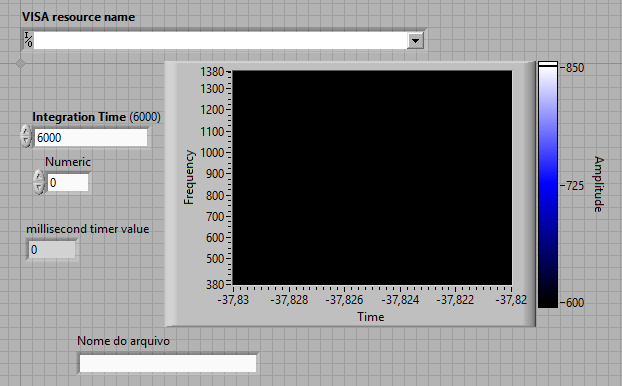
\includegraphics[width=0.7\textwidth]{imagens/fluor/painel_frontal}
				\caption{Painel frontal do programa de aquisição de dados}
				\label{fig:fluor_painelfrontal}
			\end{figure}
			
			\begin{figure}[H]
				\centering
				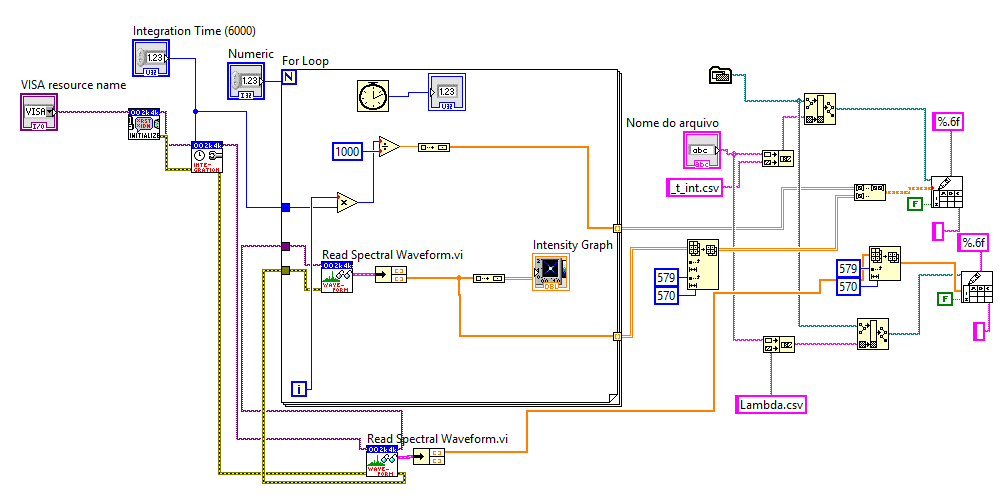
\includegraphics[width=0.7\textwidth]{imagens/fluor/gravacao_dados}
				\caption{Código fonte do programa de aquisição de dados}
				\label{fig:fluor_gravacaodados}
			\end{figure}

			% todo: colocar a pressão
			Após iniciar a aquisição de dados, acionava-se rapidamente o botão de injeção do \emph{stopped-flow}, que empurrava os êmbolos das duas seringas simultaneamente. A pressão utilizada para injeção era de XYZ Pa. Os tempos de integração e o número de pontos de aquisição variavam de acordo com o experimento. O programa gera dois arquivos, um contendo os $n$ comprimentos de onda de cada ponto medido num vetor coluna e outro continha uma matriz com os $m \times n$ pontos de aquisição, além dos $m$ tempos de aquisição, em milissegundos, na primeira coluna. A matriz resultante tem tamanho $m\times n+1$. Foi criado um mapa de cor para cada matriz.
			
			Dessa matriz, extraiu-se a coluna que continha informações em função do tempo do comprimento de onda do máximo do espectro de emissão, em 411 nm. Esse dado foi utilizado para realizar as análises quantitativas de cinética.
			
		\section{Tratamento de dados}
		
			As informações de cada amostra foram plotadas comparativamente. Notou-se que os dados eram bastante ruidosos, mas que havia uma tendência. Para melhorar a qualidade dos dados, aplicou-se o filtro de Savitzky-Golay, um para a região pré-injeção e outro para a região pós-injeção, com janelas diferentes, porém ambas de segundo grau.
			
			O filtro de Savitzky-Golay é uma maneira de se remover ruído experimental aplicando um ajuste polinomial de grau $n$ sobre uma janela de número ímpar de dados. O valor experimental do ponto médio é substituído pelo valor do ponto médio do ajuste. Isso é realizado para a curva inteira, utilizando-se, neste caso, valores constantes iguais ao primeiro/último valor para as extremidades.
		
			\subsection{Filtro Savitzky-Golay}
	\chapter{Técnicas adicionais}
		\section{Calorimetria diferencial de varredura}
		\section{Espalhamento dinâmico de luz}
		\section{Tensiometria}